\documentclass{article}
\usepackage{xcolor}
\usepackage{hyperref}

\usepackage[scaled]{helvet}
\usepackage{sectsty}
\allsectionsfont{\bfseries\sffamily}

\usepackage{listings}
\lstdefinestyle{BashInputStyle}{
  language=bash,
  morekeywords={mkdir,ls,rm,mv,cp,date,hostname,whoami,zip,unzip,rmdir,git},
  basicstyle=\small\sffamily,
%  numbers=left,
%  numberstyle=\tiny,
%  numbersep=3pt,
  frame=tb,
  columns=fullflexible,
  backgroundcolor=\color{yellow!20},
  linewidth=0.9\linewidth,
  xleftmargin=0.1\linewidth,
  literate={-}{-}1,
  keepspaces,
  showstringspaces=false,
}

\usepackage[mackeys=text,os=win]{menukeys}

\begin{document}

\noindent
{\Large \textsf{\textbf{Unix Tutorial 4.2: Collaborating via git}}}

\bigskip

Git is a powerful and popular distributed version control system for teams that are collaborating on
source code development. In this tutorial sheet, we will
investigate git commands for accessing remote repositories that are
shared between multiple users.


Although git is distributed, there are centralized repo servers like \url{https://github.com} and \url{https://bitbucket.org} that
allow easy synchronization between users.
Users \emph{publish} (\texttt{git push}) their changes to these servers, and \emph{fetch} (\texttt{git pull})
other people's changes, on shared projects.

\subsection*{Registering your ssh key}

You need to set up an ssh key-pair to use github and other online repository
sites. This allows you to do secure authentication, perhaps for
contributing to private repositories, etc.

If you don't have an ssh key pair, run the following command and press
\keys{\enter} three times (to accept the default options at the interactive prompts).

\begin{lstlisting}[style=BashInputStyle]
    $ ssh-keygen -t rsa
\end{lstlisting}
% $

This generates a public key in file \texttt{.ssh/id\_{}rsa.pub} and a private
key in file \texttt{.ssh/id\_{}rsa}. Now you need to register your public key with
github. Login at \url{https://github.com} with your username and password,
then click on your profile icon and click on the `settings' on the pop-up menu.
Now click on `ssh and gpg keys', then click the `New ssh key'  green button. Use \texttt{cat .ssh/id\_{}rsa.pub} to show the file contents, then select this and paste it into the textbox.

\begin{center}
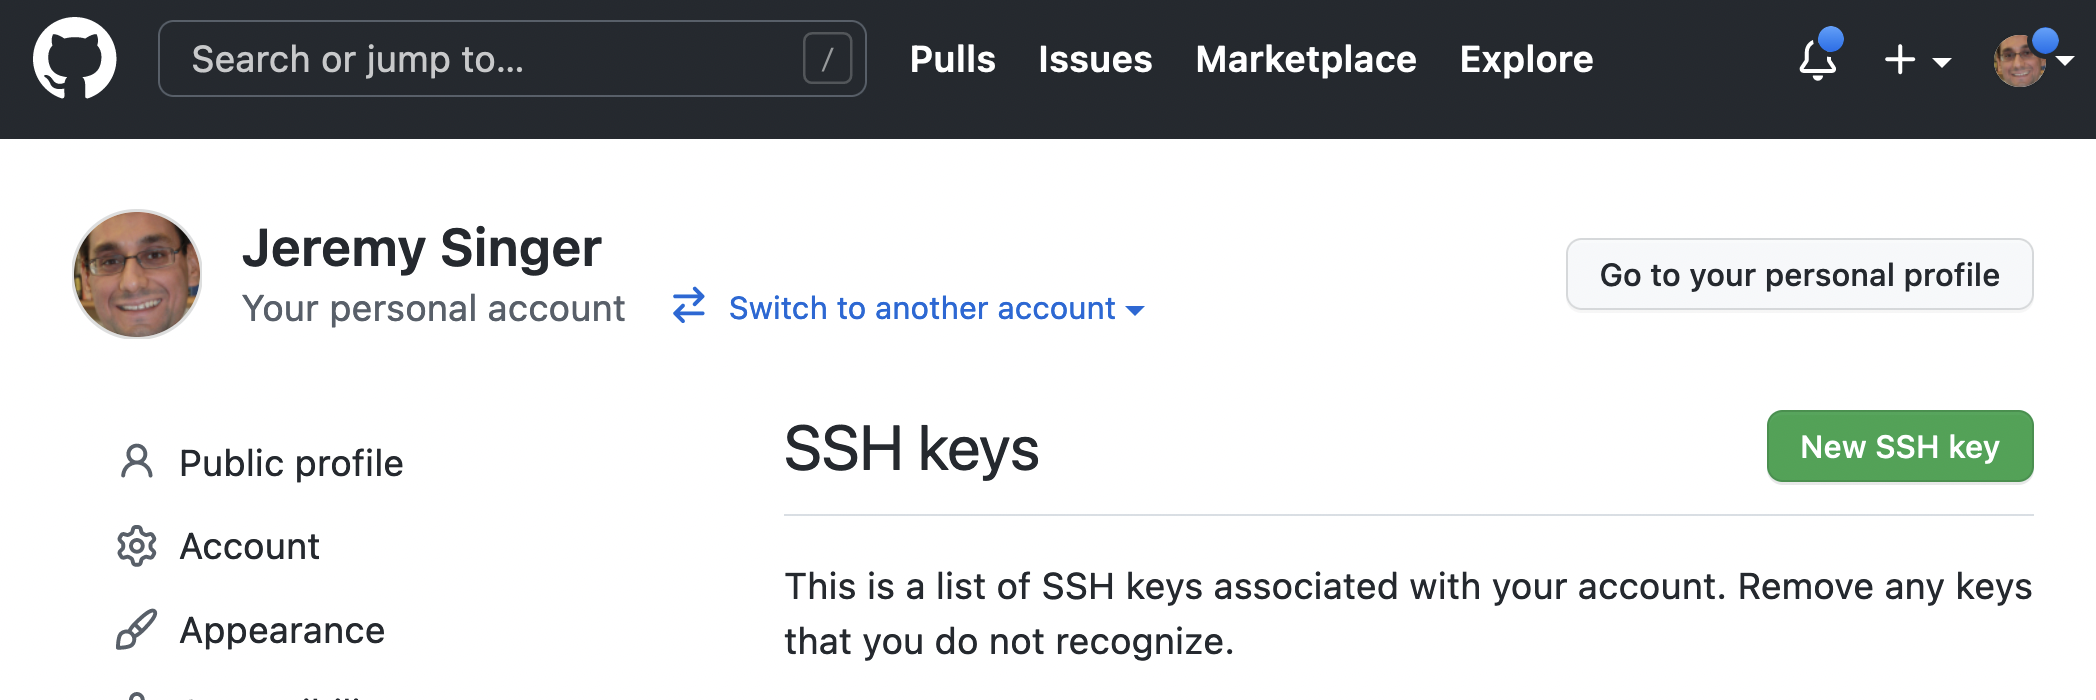
\includegraphics[width=9cm]{github_key.png}
\end{center}


\subsection*{Cloning a shared repo}

Find an `interesting' git repository you want to contribute to.
If you are working with friends, you might set up a new repo on github and
add multiple people as contributors (with read and write access).

On the other hand, if you are working on your own, it might be easier just
to \emph{fork} an existing github repo --- this copies the existing repo
into your github account so you have read and write access to this copy.
When you are logged in at the github site, find a repo --- I chose a harmless test repo at \url{https://github.com/zpqrtbnk/test-repo} and click the Fork button.

\begin{center}
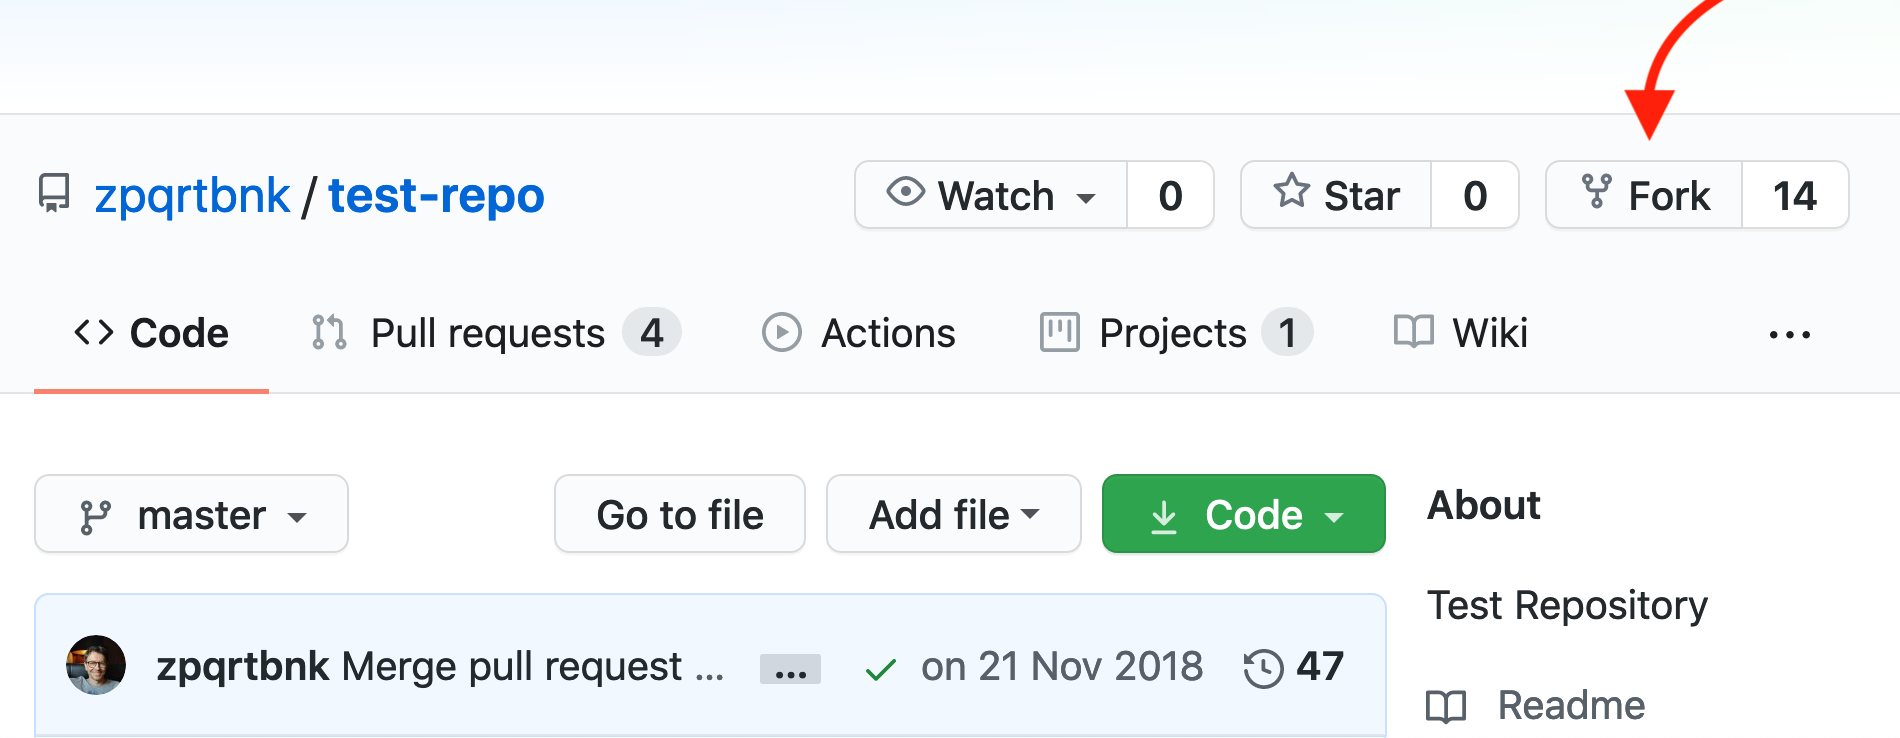
\includegraphics[width=9cm]{github_fork.png}
\end{center}

This copies the repo to your github workspace, so you end up with a repo at \url{https://github.com/YOURNAME/test-repo}.

Now you want to \emph{clone} the repo you have created. The clone operation copies the entire repo from the github server to your local machine. If it's a large repo, this might take some time.

You should clone over ssh rather than https, check the github docs for info on this. The command is:

\begin{lstlisting}[style=BashInputStyle]
    $ git clone git@github.com:YOURNAME/test-repo
\end{lstlisting}
% $


The clone command will create a new directory in the current working directory.
The new directory will have the name of the repo (\texttt{test-repo} in this example) and it is a working git repository.


\subsection*{Making changes in a shared repo}

Once you have your local copy of the git repo, \texttt{cd} into the directory and start editing files. The workflow is the same as in the previous tutorial.
Every time you make a logical, incremental change, you should \texttt{git add} the file(s) and then \texttt{git commit} the changeset with a suitable log message.

Try making a few edits to the repo you have cloned. You can also delete files with \texttt{git rm} or change their names with \texttt{git mv}. Note these are changes that need to be committed as well.

When you have made a few changes, let's try publishing these local changes back to the remote repository. The remote repo URL has been `remembered' by git --- you can see it with this command:

\begin{lstlisting}[style=BashInputStyle]
    $ git remote show origin
\end{lstlisting}
% $

OK, we use the \texttt{git push} command to send the local changes back to the remote \emph{upstream} repo:

\begin{lstlisting}[style=BashInputStyle]
    $ git push
\end{lstlisting}
% $


\subsection*{Collaborating in a shared repo}

If someone else has been working on the same upstream repository (say
a github repo that you both share) then they might have pushed their changes
upstream and you want to merge them into your local repo. This requires
the \texttt{git pull} command:

\begin{lstlisting}[style=BashInputStyle]
    $ git pull
\end{lstlisting}
% $

Note that you always need to \texttt{pull} before you \texttt{push} in a shared repo. If you try to push and your local repo is not up-to-date then git complains
and the push operation is aborted. This avoids inconsistencies in
the upstream repo.

Pulling and pushing works fine so long as git can \emph{merge} the independent changes. If both of you are working on the same lines of code in a single file then it won't be possible to auto-merge the changes --- in this case you need to manually resolve the \emph{merge conflicts}. For most people, this is their biggest git nightmare \ldots actually it's not too bad with some practice.

When you do a \texttt{git pull} you see the merge conflict reported.
The files containing conflicts have extra git lines in them, to show the
differences between your local commits and the upstream commits. The snippet below shows an example:
\begin{verbatim}
<<<<<<< COMMIT-ID:index.html
<div id="footer">contact : jeremy.singer@glasgow.ac.uk</div>
=======
<div id="footer">
 please contact Jeremy on MS Teams
</div>
>>>>>>> OTHER-COMMIT-ID:index.html
\end{verbatim}

The merge conflict is delineated with the $<<<$ and $>>>$ character sequences. The first version should be your local commit. After the $===$
you can see the conflicting commit from someone else. All you need to
do is to edit the file to remove the git char sequences and resolve the
differences. I did this:

\begin{verbatim}
<div id="footer">
 please contact Jeremy on MS Teams or by email
</div>
\end{verbatim}

Then we go through the regular sequence:


\begin{lstlisting}[style=BashInputStyle]
    $ git add index.html
    $ git commit
\end{lstlisting}
% $

When you commit, git will say something like `it looks like you are resolving a
merge conflict' --- and auto-generate a log message for you. Then you can push the merged code back to the centralized repo.


\subsection*{Other useful commands}

If multiple developers are working on independent features, often they want
to use separate \emph{branches} to localise their changes and to prevent
frequent merge conflicts.

If you want to highlight a particular commit id (perhaps it is a beta release or something) then you can \emph{tag} the version just after you have committed it:

\begin{lstlisting}[style=BashInputStyle]
    $ git tag -a v1.0 -m "Release version 1.0"
\end{lstlisting}
% $

Next time you run a \texttt{git log} then you will see the tags associated with the commits. You can also list all the tags with \texttt{git tag} without any arguments.


Do you see who has made the most recent change to each line of an individual file? The intriguingly named \texttt{git blame} command is useful here.


\begin{lstlisting}[style=BashInputStyle]
    $ git blame file.txt
\end{lstlisting}
% $

Can you see how to run this command, combined with some \texttt{cut} and \texttt{sort -u} and \texttt{grep -c} to work out who has contributed the most lines of code in your team project repo?



\section*{Further Reading}

There are lots of online resources and tutorials for git.
Try the selection at: \url{https://git-scm.com/doc}.
There is a nice (if slightly obscene) graphical guide at 
\url{https://rogerdudler.github.io/git-guide/}.


\end{document}
